\chapter{Utilities}

\section{Lowenstein Script} \label{Sec:Lowenstein}
This is a script provided for easy augmentation of a given silicate structure subject to the 
Lowenstein Rule for zeolites.  Given a single unit cell of arbitrary shape, this script randomly inserts Aluminum
atoms until the specified Lowenstein Ratio (\# Si / \# Al) is achieved.  Acceptable target ratios are on the range
of [1.0, inf).

\subsection{Usage} \label{sec:Usage}
To use the Lowenstein\_Script.f90: compile the script, open the executable, and run the program.
Sample code would be:

\texttt{> gfortran Lowenstein\_Script.f90 -o Lowenstein\_Script; ./Lowenstein\_Script} \\

Following this, the user is presented with four sequential prompts:

\texttt{> Enter the name of the initial data file:}  \\
\texttt{> Enter the desired final Lowenstein Ratio ( [1.0, inf)): } \\
\texttt{> Use random initial seed? (Y/N): }\\
\texttt{> Enter the name of the output file: } \\


To reproduce a structure with an identical Lowenstein ratio as example\_ratio\_2\_1.xyz (which has a Lowenstein ratio 
of 2), one might respond to the prompts with:

\texttt{> Enter the name of the initial data file:  example.pdb  }\\
\texttt{> Enter the desired final Lowenstein Ratio ( [1.0, inf)):  2.0  }\\
\texttt{> Use random initial seed? (Y/N): Y  } \\
\texttt{> Enter the name of the output file: output\_file.xyz  } \\

The file output\_file.xyz will contain your new structure with a Lowenstein Ratio of 2.0 and will 
be placed in the current directory.


\subsection{Input} \label{sec:Input}
The script reads the first line of the .pdb according to the following format code:

\begin{lstlisting}[firstnumber=184, caption=Lowenstein\_Script.f90]
    350 FORMAT(8X,2(F8.4,1X),F8.4,3(F7.3))
\end{lstlisting}

This data is stored in variables corresponding to the A, B, C, $\alpha$, $\beta$, and $\gamma$   
parameters of a unit cell and is required for the script to function.

The next line of code in the file should contain information pertaining to atom number 1 of the unit cell, and 
all other atoms should immediately follow on distinct lines, uninterrupted until the 'END' statement of the file is reached.

Information for each atom that should be present on their respective line includes:
\begin{itemize}
\item x-coordinate
\item y-coordinate
\item z-coordinate
\item element
\end{itemize}

The format code that reads in this information is given by:

\begin{lstlisting}[firstnumber=231, caption=Lowenstein\_Script.f90]
    450 FORMAT(31X,3(F7.3,1X),21X,A2)
\end{lstlisting}

For a direct example of acceptable input format, see:  /Scripts/Lowenstein/example.pdb

\section{Input File GUI} \label{Sec:GUI}
This script provides a graphical user interface with which the user may create input files for use in simulations.  The GUI is written
 in Python and uses the wxWidgets for Python module, which may be found at:   

http://wxpython.org/download.php 

\section{Generator of MCF files}
\label{utility:mcfgen}

The script \texttt{mcf\_gen.py} is a tool that aims to ease the setup of MCF files from scratch (see section \ref{sec:MCF_File} to learn more
about MCF files), as the generation of these files by hand can be error prone. 
In this section, a pentane MCF file will be generated to demonstrate the use of this tool.
The Transferable Potentials for Phase Equilibria (TraPPE) force field will be used to represent the pentane molecular interactions. 
This force field involves a pairwise-additive 12-6 Lennard-Jones potential to represent the dispersion-repulsion interactions. Additionally, bond angles and dihedral angles are represented through
harmonic and OPLS functional forms, respectively. Bond lengths are kept constant. The force field mathematical
expression becomes

\begin{align*}
U = \sum_{angles} K_\theta(\theta-\theta_0)^2 +
\sum_{dihedrals} \frac{1}{2}K_1[1+cos(\phi)]+\frac{1}{2}K_2[1-cos(2\phi)] + \frac{1}{2}K_3[1+cos(3\phi)]+\frac{1}{2}K_4[1-cos(4\phi)] + \\
\sum_{i} \sum_{i>j} 4 \epsilon_{ij} \left [  \left ( \frac {\sigma_{ij}} { r_{ij} }\right )^{12} - \left ( \frac {\sigma_{ij}} { r_{ij} }\right )^{6}\ \right ]
\end{align*}

First, generate (or obtain) a PDB file or a CML file. To generate a PDB or CML file, 
software such as Gaussview or Avogadro can be used. Alternatively, PDB files can
be downloaded from the internet (e.g. www.rcsb.org). In this example, a pentane PDB file using the 
program Gaussview v5.08 will be generated, as shown below. \\

%After launching the Gaussview interface, click on the ``Element Fragment'' button located on the upper-left corner of the
%window.
%
%
%\begin{figure}[h]
%\begin{center}
%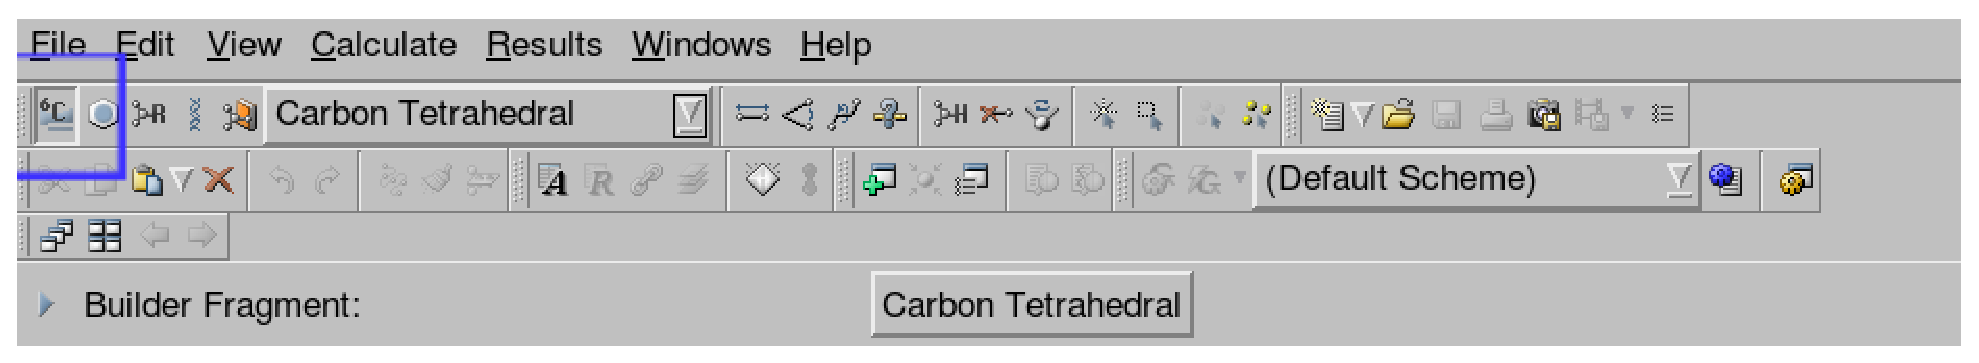
\includegraphics[height=1in]{gaussian1final.eps}
%\end{center}
%\end{figure}
%
%A periodic table will appear. Click on the ``Carbon'' button. 
%
%\begin{figure}[h]
%\begin{center}
%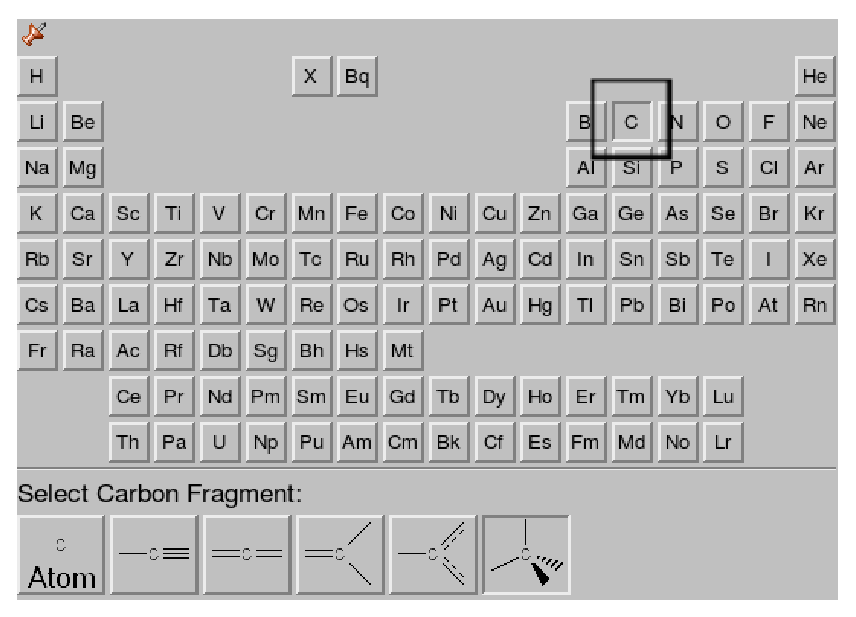
\includegraphics[height=3in]{gaussian2final.eps}
%\end{center}
%\end{figure}
%
%Click on the main workplace to insert the first $CH_4$ fragment.
%To increase the chain length, click on a hydrogen attached to the carbon. 
%
%\begin{figure}[h]
%\begin{center}
%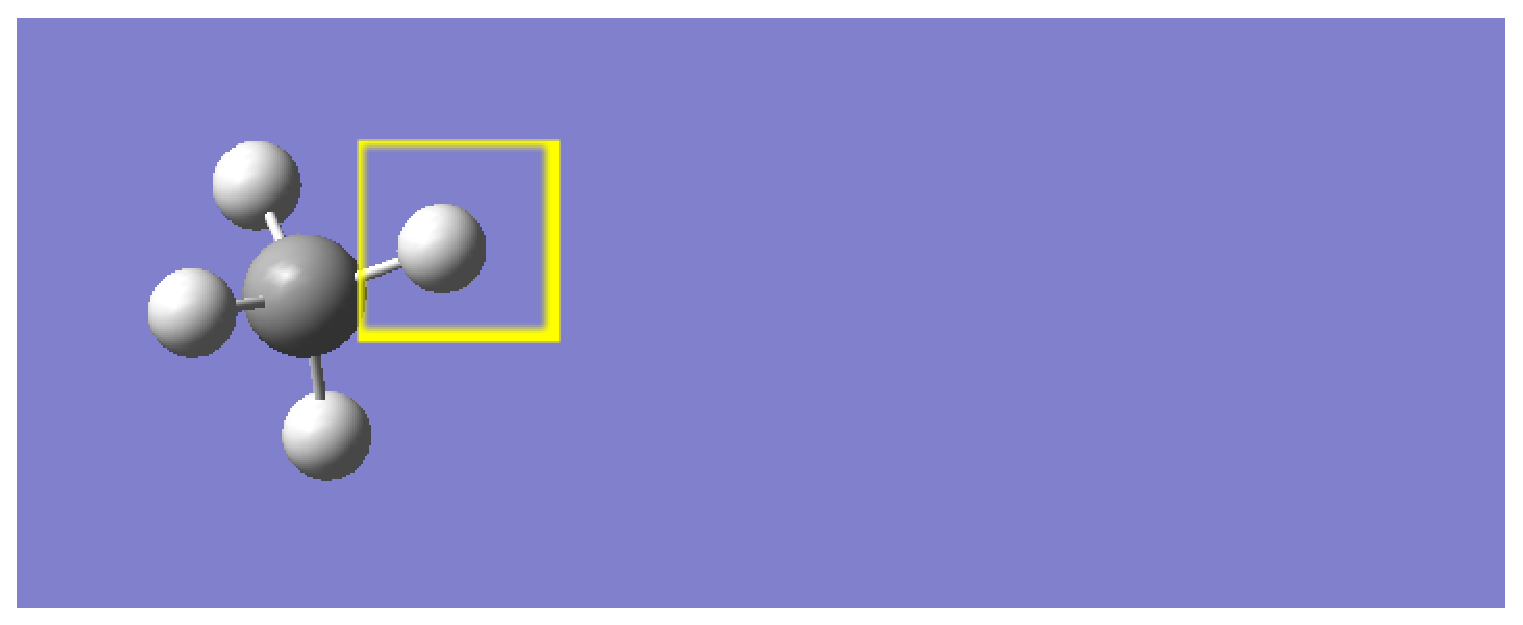
\includegraphics[height=2in]{gaussian3final.eps}
%\end{center}
%\end{figure}
%
%The final pentane structure should look something like this
%
%\begin{figure}[h]
%\begin{center}
%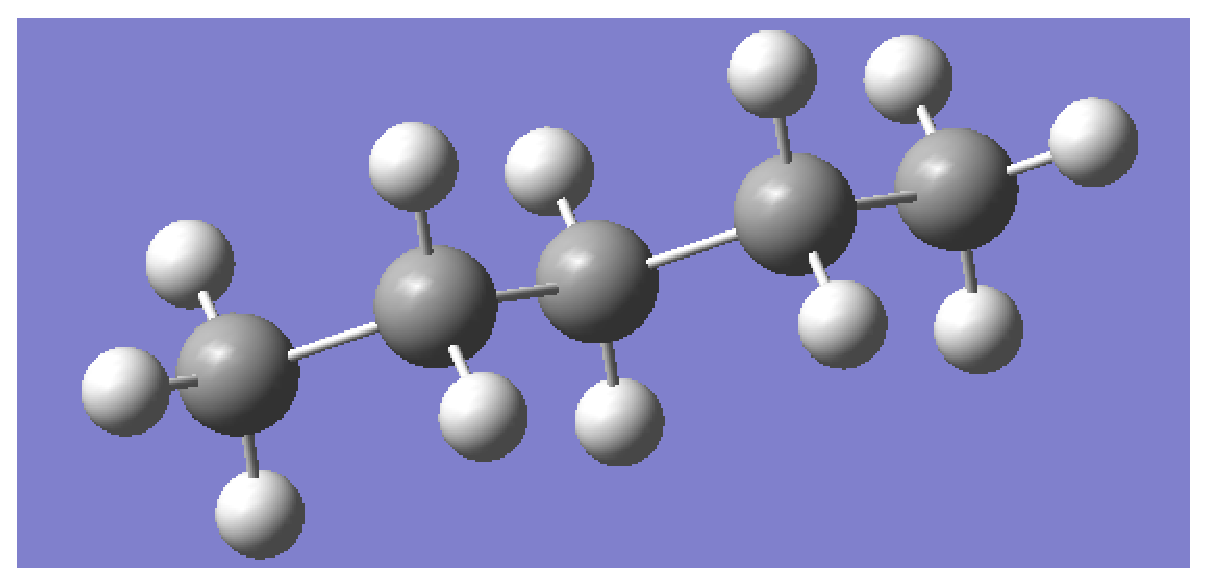
\includegraphics[height=2in]{gaussian4final.eps}
%\end{center}
%\end{figure}
%\vspace{3in}
%Right click on any place of the workplace, select the option builder and then
%select delete atoms.
%
%\begin{figure}[h]
%\begin{center}
%\includegraphics[height=2.5in]{gaussian5final.eps}
%\end{center}
%\end{figure}
%
%Click on all the hydrogen atoms to delete them 
%
%\begin{figure}[h]
%\begin{center}
%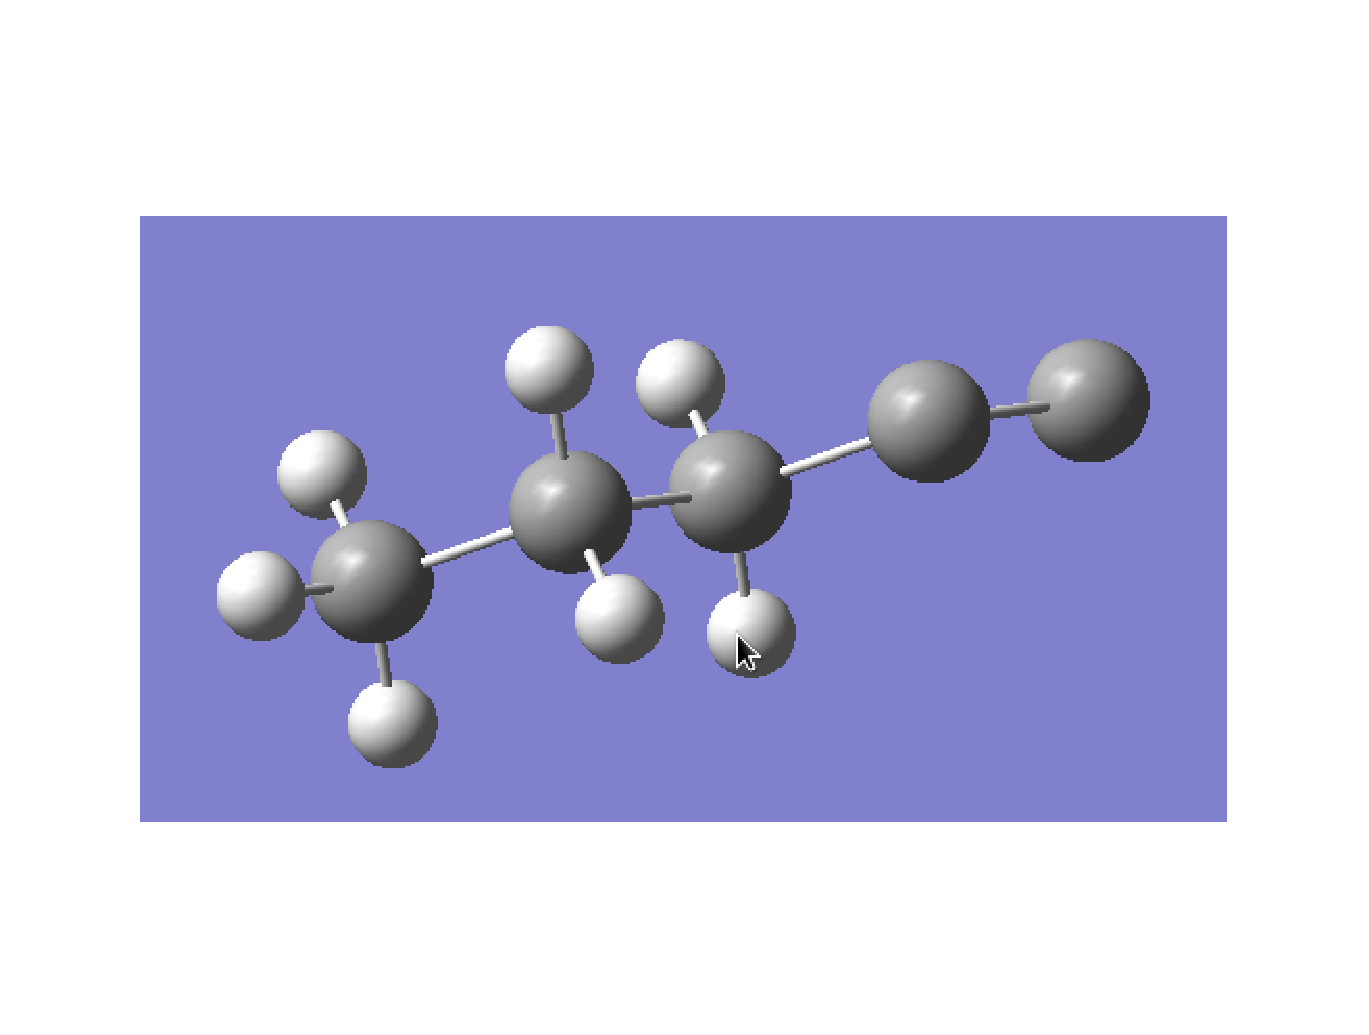
\includegraphics[height=2.5in]{gaussian7final.eps}
%\end{center}
%\end{figure}
%
%\vspace{3in}
%Go back to main menu, click on File - Save.
%
%\begin{figure}[h]
%\begin{center}
%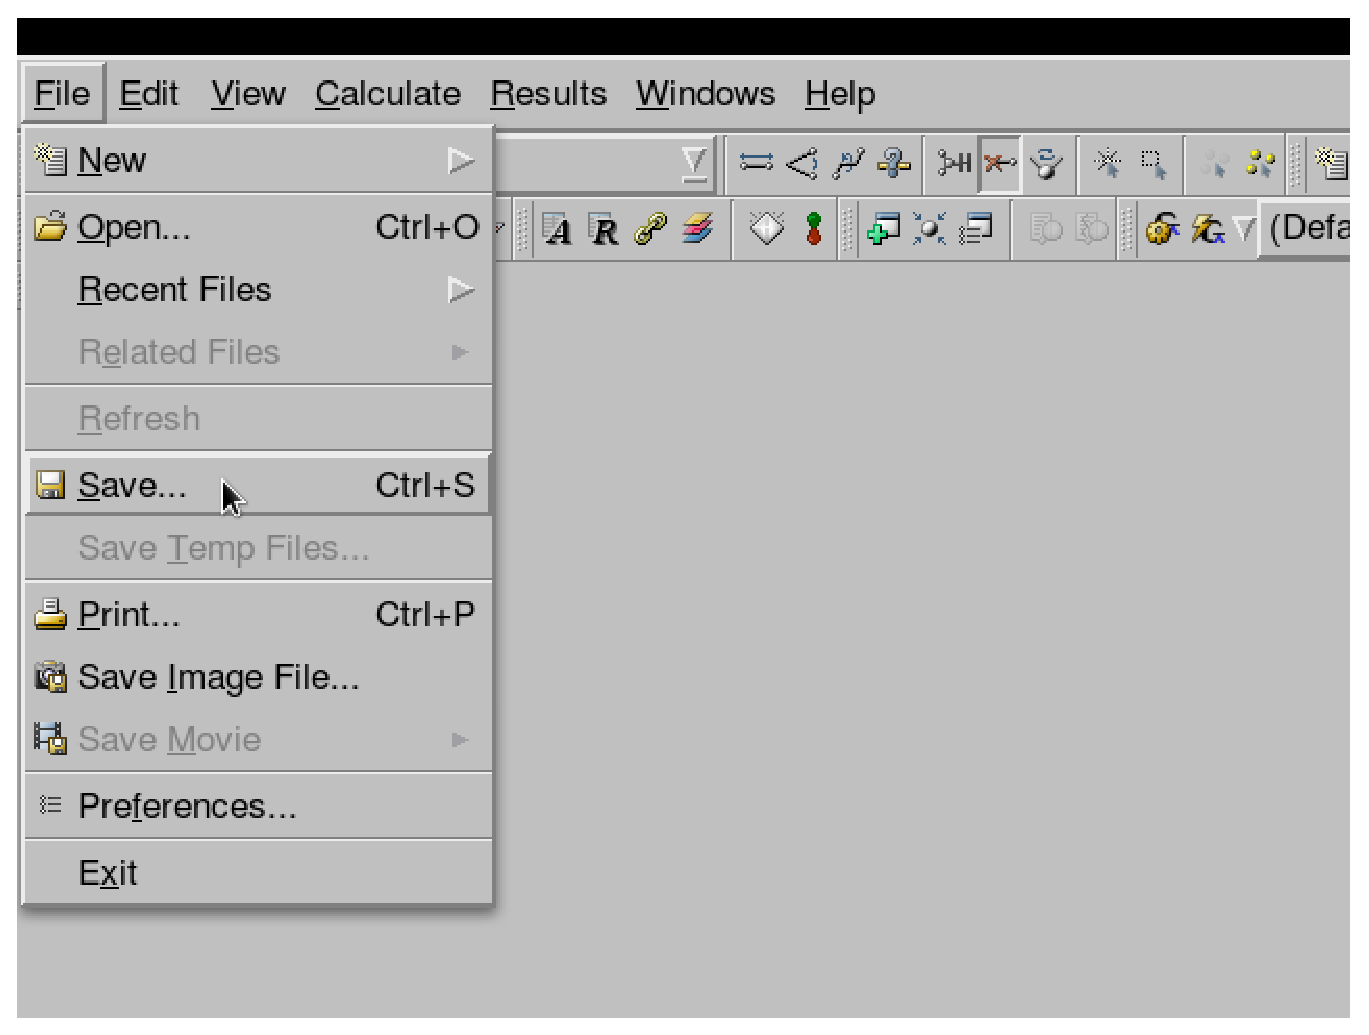
\includegraphics[height=2.5in]{gaussian8final.eps}
%\end{center}
%\end{figure}
%
%Type the name of the file and select PDB as the file type from the bottom menu.
%
%\begin{figure}[h]
%\begin{center}
%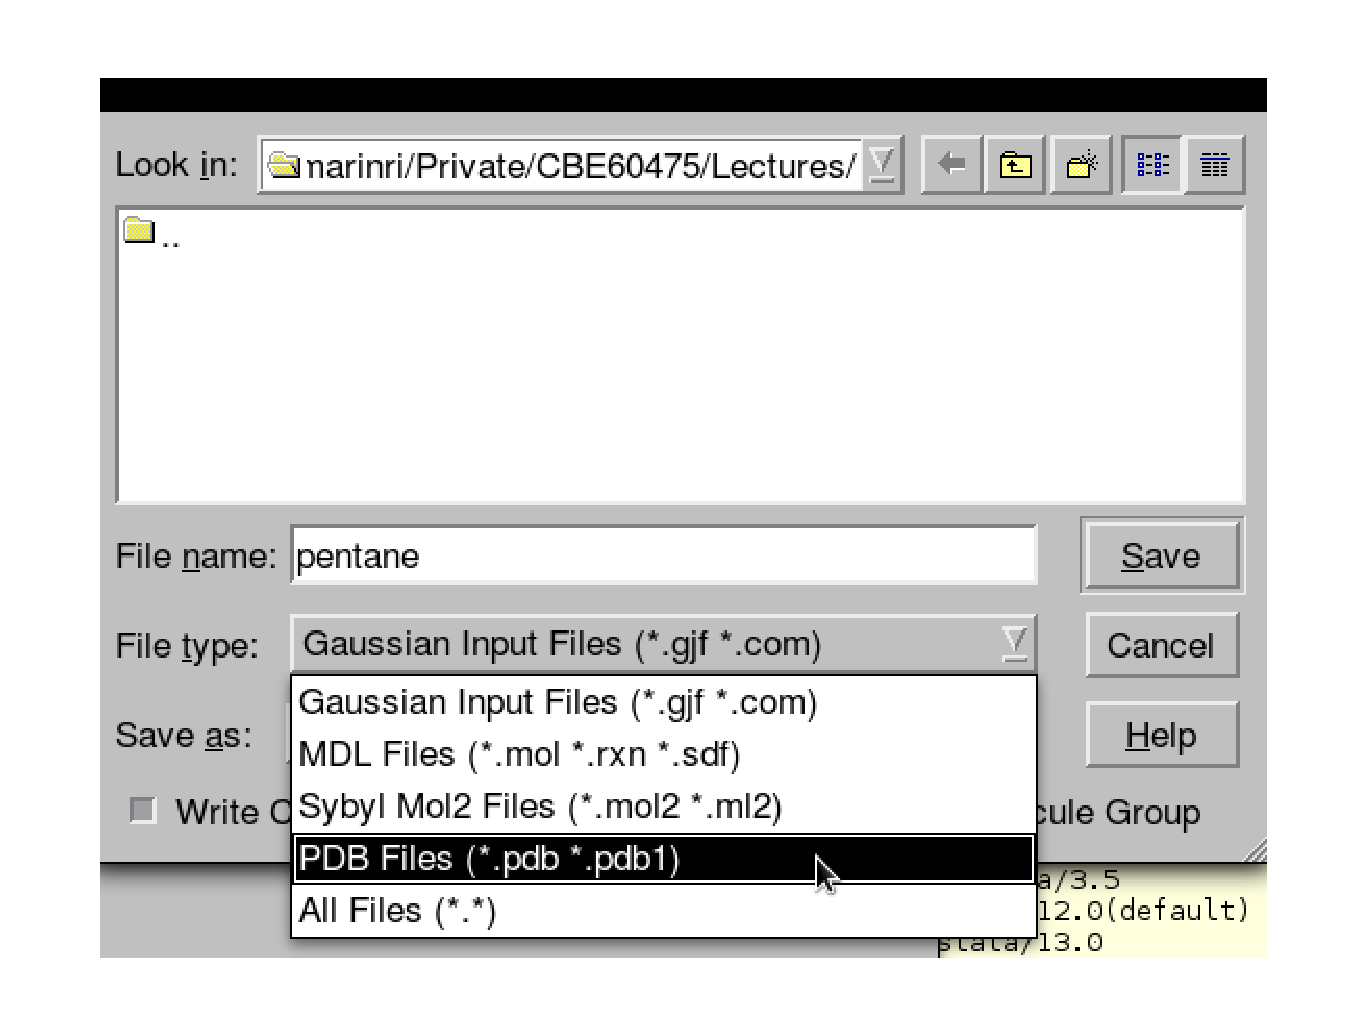
\includegraphics[height=2.5in]{gaussian9final.eps}
%\end{center}
%\end{figure}
%
%\vspace{3in}
%Close Gaussview. Back in the terminal, open the PDB file using your favorite text editor.

\begin{figure}[h]
\begin{center}
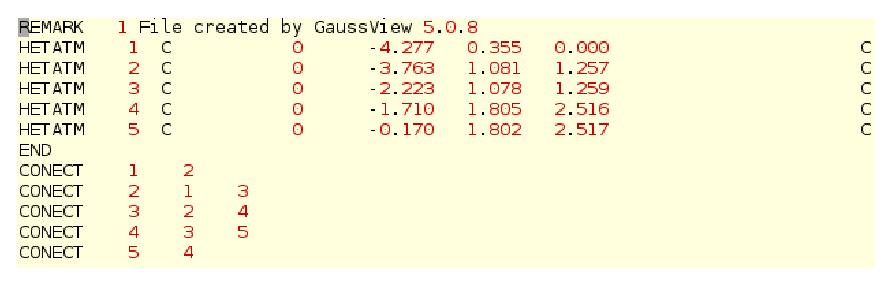
\includegraphics[height=1in]{pdbfile_final.eps}
\end{center}
\end{figure}

Append a column containing the atom types.

\begin{figure}[h]
\begin{center}
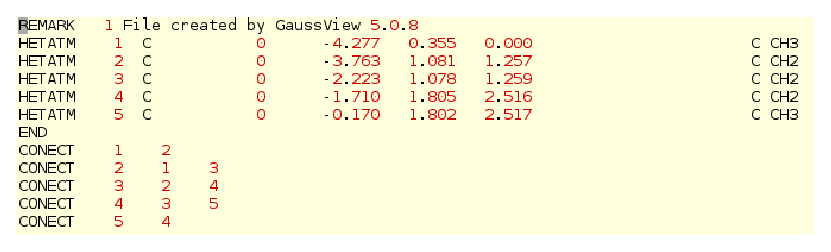
\includegraphics[height=1in]{pdbfile_edited_final.eps}
\end{center}
\end{figure}

Avogadro v1.1.1 can also be used to generate CML files. The procedure is analogous 
to the one previously presented for Gaussview.

\begin{figure}[h]
\begin{center}
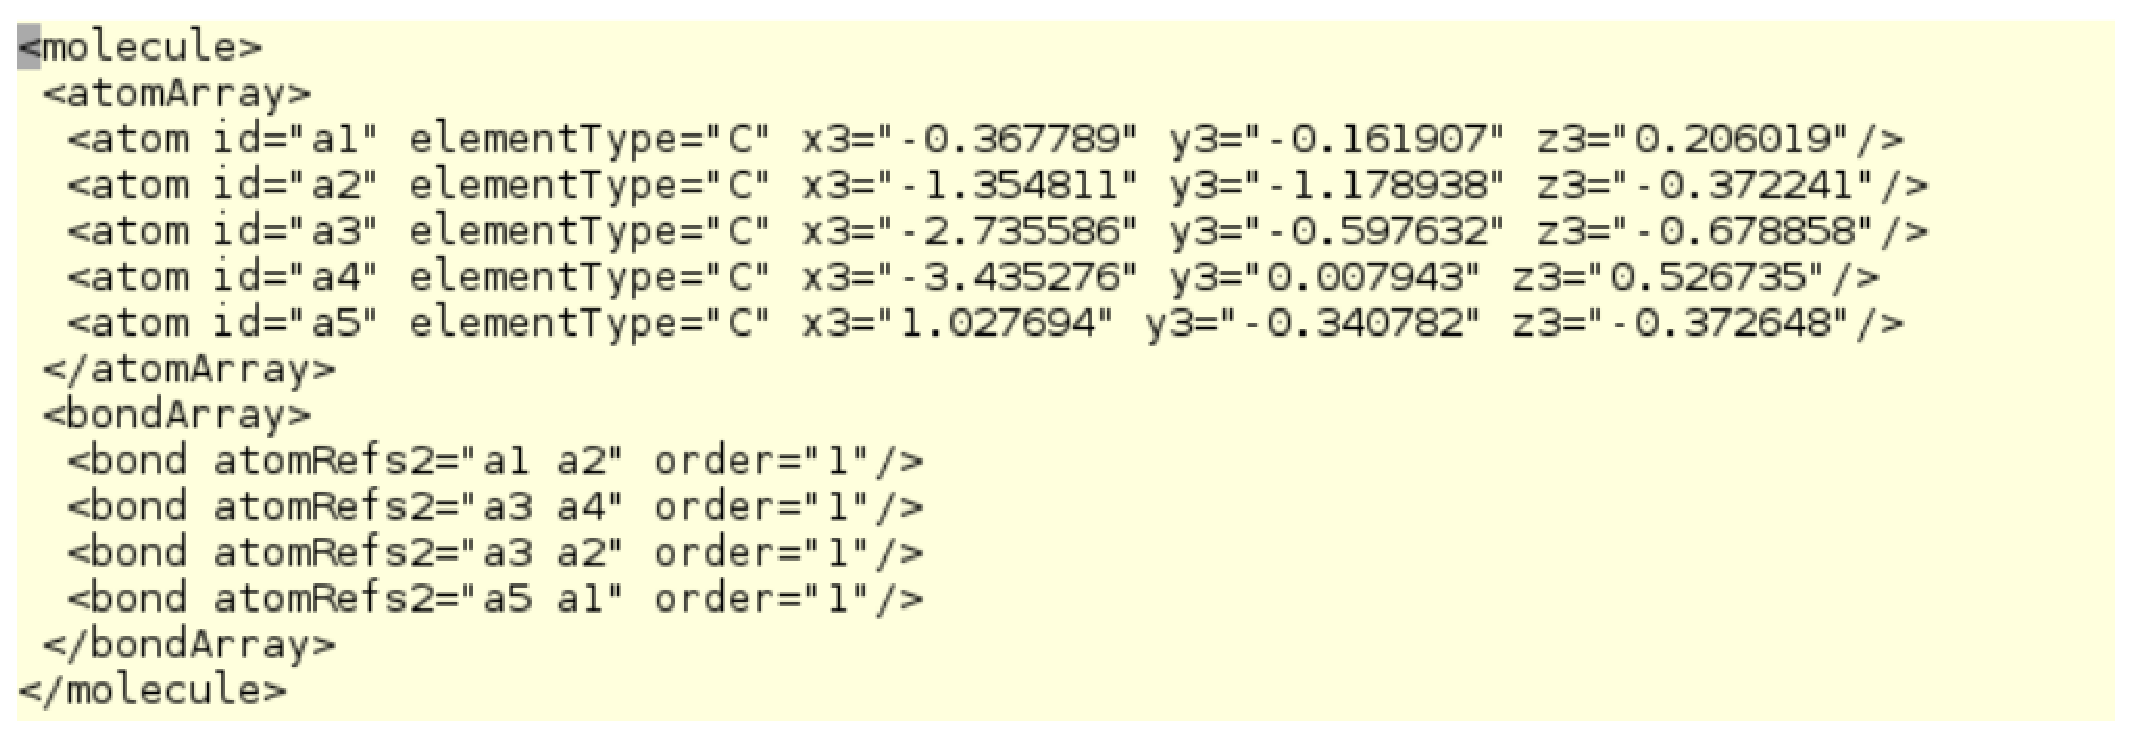
\includegraphics[height=1.5in]{pentane_cml.eps}
\end{center}
\end{figure}

\vspace{3in}
Modify the pentane united atom CML file. Note that the atom type is appended as a last
column between quotation marks.

\begin{figure}[h]
\begin{center}
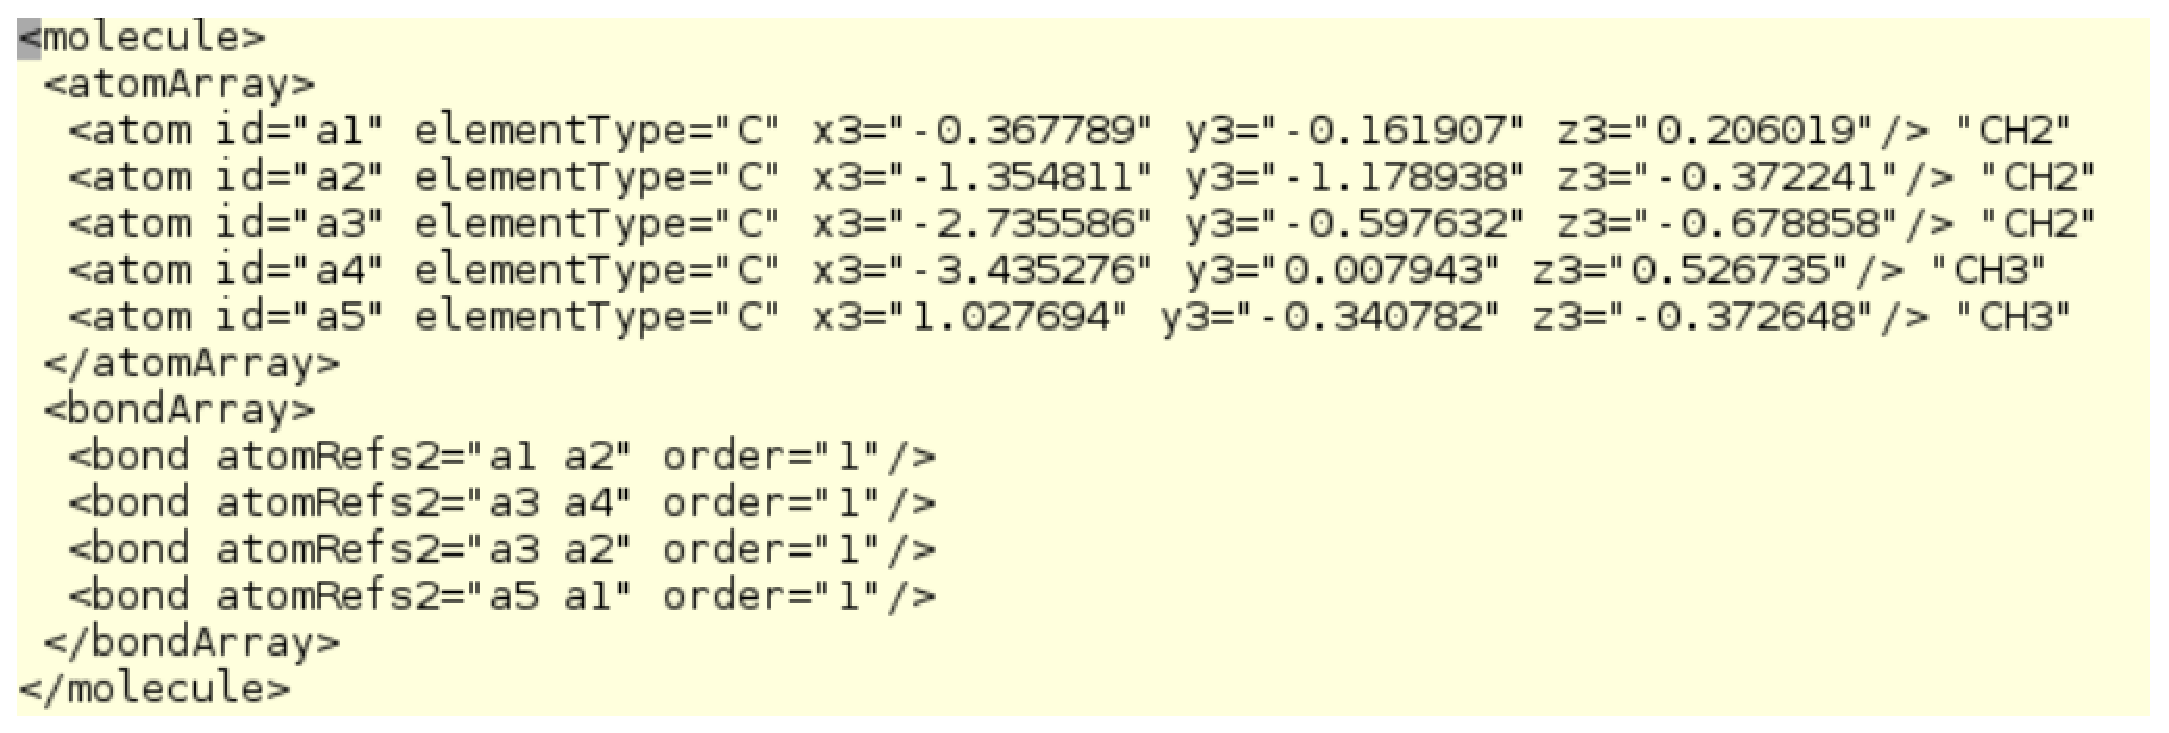
\includegraphics[height=1.5in]{pentane_cml_modified.eps}
\end{center}
\end{figure}

In the terminal, run the following command:\\
\texttt{>python mcfgen.py pentane.pdb --ffTemplate}

This command will create an .ff file. The first three sections of the FF file are displayed next. 
Do not modify these.

\begin{figure}[h]
\begin{center}
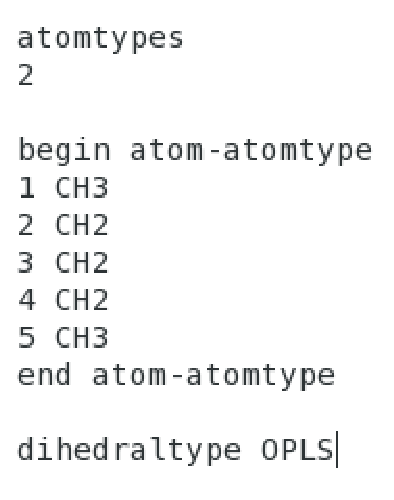
\includegraphics[height=2in]{top_ff.eps}
\end{center}
\end{figure}

The force field parameters for non-bonded (not shown), bonded, angle, dihedral (not shown)
and coulombic interactions (not shown) must be entered next to the corresponding keyword.
For example, the angle type CH3 CH2 CH2 has an angle of 114.0. This value must be placed
next to the ``Angle'' keyword.

\begin{figure}[h]
\begin{center}
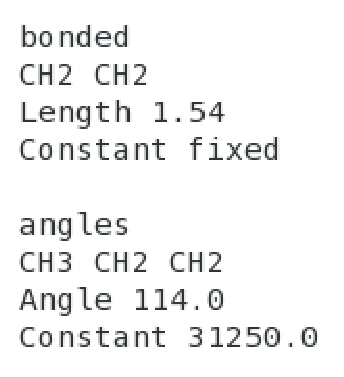
\includegraphics[height=1.5in]{body_ff.eps}
\end{center}
\end{figure}

\vspace{3in}
For more examples of filled ff files, please refer to the examples contained in the /Scripts/MCF\_Generation/ directory. Using the
filled .ff file, run: \\

\texttt{> python mcfgen.py pentane.pdb} \\

Check the file newly created pentane.mcf for any possible errors. This example can be found in the directory 
/Scripts/MCF\_Generation/PDB/

\section{Generate library of fragment configurations}
\label{utility:libgen}

The goal of the script \texttt{library\_setup.py} is to automate the generation of fragment libraries.
As a starting point, the script requires the simulation input file, and the MCF and PDB 
files for each of the species. To run this script, type \\

\texttt{> library\_setup.py \$PATH\$/cassandra.exe input\_file.inp pdbfilespecies1.pdb pdfilespecies2.pdb ...} \\

This script will create the necessary files to create the fragment libraries. It will also run Cassandra 
to generate these libraries, whose location will be at \\

\texttt{/species?/frag?/frag?.inp} \\

where '?' refers to the species number, for example, species 1, species 2 etc. \\

Note that the script overwrites the section of the input file where 
needed (i.e. \# Frag\_Info) with the aforementioned directory locations.
